
\documentclass{ar-1col}


\usepackage[comma]{natbib}
\usepackage{url}
\setcounter{secnumdepth}{4}

% Metadata Information
\jname{Xxxx. Xxx. Xxx. Xxx.}
\jvol{AA}
\jyear{2020}
\doi{10.1146/((please add article doi))}



\begin{document}

% Page header
\markboth{Hassan and Zhang}{The Economics of Currency Risk}

% Title
\title{Title: Subtitle}


%Authors, affiliations address.
\author{Tarek A. Hassan,$^1$ and Tony Zhang$^2$
\affil{$^1$Department of Economics, Boston University, Boston, USA,  02213; email: thassan@bu.edu}
\affil{$^2$Board of Governors of the Federal Reserve System, Washington, USA, 20551; email: tony.zhang@frb.gov}}



\title{The Economics of Currency Risk\thanks{}}



\begin{abstract}
  This article reviews the literature on currency risk with a focus on
  its macroeconomic origins and implications. A growing body of
  evidence shows that countries with safer currencies enjoy
  persistently lower interest rates, a lower required return to
  capital, and accumulate relatively more capital than countries
  international investors perceive as risky. While earlier research
  has focused mainly on the role of currency risk in generating
  violations of uncovered interest parity and other financial
  anomalies, more recent evidence also points to important
  implications for the allocation of capital across countries, the
  efficacy of exchange rate stabilization policies, the sustainability
  of trade deficits, and the spill-over of shocks across borders.
\end{abstract}


%Keywords, etc.
\begin{keywords}
keywords, separated by comma, no full stop, lowercase
\end{keywords}
\maketitle

%Table of Contents
%\tableofcontents


\section{Introduction}


A key tenet in economics is that the degree to which firms should be
willing to invest in a given project depends crucially on the required
rate of return to capital: A price-taking firm should install just
enough capital so that the marginal product of capital, $MPK_i$, equals
the required rate of return to capital,$r_i$, 
\begin{equation}
    MPK_i=\underbrace{r^f+RP_i}_{r_i}.
    \label{eq_one}
\end{equation} 
This equation is the point of departure for many classic questions in economics. Students of asset
pricing are taught that a firm's $r_i$ has two components; a risk-free
part, $r^f$, and a risk-premium, $RP_i$, that depends on the firm's
risk characteristics. One of the classic puzzles in asset pricing is
why $RP_i$ is so large relative to $r^f$ (the equity premium puzzle).
Monetary economists are interested in the Federal Reserve's power to increase or decrease investment by
manipulating $r^f$, while students of economic growth often take
differences in $MPK_i$ as a measure of inefficiencies in the
allocation of capital across countries, sectors, and firms.

In this article we argue that recent insights from the study of
currency risk premia have important lessons for how we should think
about equation (\ref{eq_one}), and by extension, for its key
applications in asset pricing, macroeconomics, and economic growth.
The simplest, and perhaps and most important, of these lessons is that
countries differ dramatically in their risk-free interest rates. These
differences in risk-free interest rates are large (on the same order
of magnitude as the equity premium puzzle), appear to be highly
persistent over time (lasting for decades rather than years), and
cannot be explained by predictable depreciations, government default,
or differences in inflation rates. Instead, these differences in
interest rates appear intimately linked to the risk characteristics of
the country's exchange rate, and to its exchange rate regime.

\begin{figure}
    \centering
    \caption{Risk-free Interest Rates}
    \includegraphics[width=0.7\textwidth]{Exhibits/Figure_FP12M_JPYNZD.pdf}
    \label{fig:fp}
\end{figure}
Figure \ref{fig:fp} shows the difference in the risk-free interest rates of the
New Zealand Dollar and the Japanese Yen as an example (we will discuss
below how one can measure such risk-free rates and compare them across
countries). The Figure shows that the New Zealand dollar had a higher
risk-free rate than the Japanese Yen in \textit{every} month between
January 1997 and July 2020. On average, this difference was about 
4.39pp on an annualized basis. When we adjust for movements in exchange rates over
the period, the difference in returns on the two countries currencies
is XXpp -- meaning that a US investors who borrowed in Yen and lent in
New Zealand Dollars on average made a return of XX percent over this
period. (For comparison, the equity premium on US stocks was about
XXpp during the same period.)

We now know that such highly persistent differences in interest rates,
similar to those between New Zealand and Japan, are common in the
data, even among developed economies. These large differences in
interest rates do not appear to be equalizing over
time and translate into large differences in returns investors can
earn when investing in these currencies.

Why would $r^f$ differ permanently across countries? The emerging
consensus in the literature is that the most likely explanation are
currency risk premia -- the idea that some currencies are safer
investments than others. 

A useful way of thinking about this problem
is to take the perspective of a retail investor in a third country, say in Hong Kong.
As is common in many countries, Hong Kong-based banks regularly offer savings accounts denominated in multiple currencies, so that our fictitious investor might have the option to invest in yen at a deposit rate of 0.1\% or in New Zealand Dollars at a rate of 3.0\%. How might she decide between these two options? Since both accounts are with the same bank, any likelihood of sovereign default is irrelevant. Similarly, our Hong-Kong based investor does not care about inflation in these two faraway countries. Instead, the only relevant factors for her choice between these two investment is the difference in interest rates and the stochastic behavior of the yen-to New Zealand dollar exchange rate. 

Because changes in exchange rates are largely unpredictable over short horizons, our investor should not expect either currency to depreciate over the coming year, leaving only one relevant consideration: covariance. Which of the two currencies does our investor trust to retain value in a possible recession or crisis? Intuitively, she might think that Japanese yen are a safer bet -- and she would be right. Along with a number of other so called ``safe-haven currencies,'' the Japanese yen tends to appreciate relative to the New Zealand dollar during large international recessions and crises. If yen are a safer store of value, it might make sense to accept a lower deposit rate. That is, international investors might be willing to lend at lower rates in currencies they expect to retain value when times are bad. 

As it turns out, this simple intuition has a lot of support in the
data from international bond and derivatives markets. For example, a seminal paper by \citet{LustigVerdelhan2007}
shows that currencies with low interest rates on tend to appreciate
when US consumption growth is low, and depreciate when US consumption
growth is high. That is, there is direct evidence that currencies with
low interest rates appreciate when times are bad for US consumers, making these currencies a
safer store of value for investors.

In addition to this empirical evidence, the theoretical work on
currency risk has identified a number of theoretical reasons to expect
the emergence of safe-haven currencies and long-lasting differences in
interest rates. In a nutshell, currency risk premia arise naturally in
a wide range of international macro models. For example, \citet{Hassan2013}
shows that simply allowing for some economies to be larger than others
within a standard international real business cycle model is
sufficient to generate long-term differences in interest rates between
countries, because the currencies of larger countries tend to
appreciate when world-wide output is low. That is, even within the
most canonical, frictionless, international macro models currency
risk premia tend to arise naturally in equilibrium. Other authors have
similarly pointed to the emergence of currency premia in models with
intermediary capital constraints, trade costs, and differences in
resource endowments, among others.


We survey the rapidly growing empirical and theoretical literature on
currency risk premia in detail in sections XX and XX. Because the
initial focus of this literature was mainly on resolving asset pricing
anomalies, many of its key papers tend to use technical finance language.
For this reason we attempted to keep this review as non-technical as
possible, focusing as much as possible on the underlying economics.

A major difficulty this literature shares with a broader literature in
asset pricing is that models with conventional preferences tend to
produce risk premia that are quantitatively small. That is, although a
number of papers have identified compelling reasons why, for example,
the interest rate in Japan should be lower than that in New Zealand,
most of these models suggest that it should be lower by something on
the order of 0.04pp rather than the 4.23pp we measure in the data. In
this sense, the literature is running into a quantitative ``interest
differential puzzle,'' which is in some ways analogous to the equity
premium puzzle. Both puzzles fundamentally struggle with the
prediction of models with standard preferences that risk premia should
be small given the relatively small aggregate variation in consumption
growth we measure in the data. Quantitative research on currency risk
is thus a major area for future research.


Although the literature on currency risk premia has proliferated in
recent years, it has perhaps been less successful at making clear the
relevance of its findings beyond the financial context, a gap we hope to
partially fill with this article.

Perhaps the most immediate implication of currency premia for the real
economy is for capital accumulation: If countries differ persistently
in $r^f$, then those with higher interest rates have a persistently
higher cost of capital and thus, according to (\ref{eq_one}) should
produce with relatively less capital. Returning to our example from
Figure \ref{fig:fp}, it turns out that indeed the capital-to-output ratio K/Y in
New Zealand is 22 percent lower than in Japan, suggesting that,
indeed, the marginal product of capital is larger in New Zealand than
it is in Japan. More generally, countries with persistently higher
interest rates appear to have higher marginal products of capital in
the long-run. This simple insight has direct implications for several
strands of the macroeconomic literature.

The first is for the so-called Lucas-puzzle \citep{Lucas1990}, which
posits that, over long periods of time, capital-to-output ratios do not appear to be equalizing across countries, and in particular, not enough capital appears to be flowing to developing nations to equalize the marginal product of capital. If indeed some currencies are permanently riskier than others, then currency risk is one possible factor preventing such equalization.

A second, related, implication is for a large literature that focuses on assessing the efficiency of the allocation of capital across countries \citep{HallJones1997, CaselliFeyrer2007}. A basic assumption in this literature is that $r^f$ is equalized across countries, so that systematic deviations from this required rates can (partially) be attributed to inefficiencies. However, if there are fundamental (efficient) reasons for $r^f$ to differ due to differing currency (and country) risk characteristics, some of these calculations will have to be modified.

Third, an active literature in international finance has studied the propensity of firms and countries to borrow in foreign currency \citep{DuSchreger2016, KalemliOzcanetal2019}. If lending in a low-interest-rate currency is safer than lending in a high-interest-rate currency, then the opposite is true for borrowing. That is, firms that borrow in dollar, yen or another safe-haven currency may be loading up on systematic risk -- a price they pay for enjoying lower rates.

Aside from issues surrounding capital accumulation and investment, long-lasting differences in interest rates across countries may also change how we think about two major XXX. The United States and a number of other countries is running a persistent current account deficit, the sustainability of which depends crucially on its ability to borrow cheaply in international markets \citep{GourinchasRey2007}. If there are fundamental economic reasons why the US dollar is a safer currency than many others, then lower US interest rates are here to stay, potentially enabling the United States to sustain trade and current account deficits in perpetuity.

If there is indeed something to this story, it changes how we think
about central issues in macro.

 4) Exchange rate regimes and risk 5)
Dynamics, capital flows and risk

FIXMETH CONTINUE ONCE WE KNOW HOW WE END THE PAPER

\section{Risk-free Interest Rates, the Carry Trade, and Failures of Uncovered Interest Parity}

Much of the early on currency risk focused on understanding three puzzling empirical facts in currency markets. The first is that that regressions of changes in the exchange rates on differences in interest rates yield a coefficient smaller than one, suggesting that, on average, high-interest-rate currencies do not depreciate enough to wipe out any differences in interest rates (Bilson, 1981; Fama, 1984). The second is that investors in the \textit{Carry Trade} seem to be making money on this fact by borrowing in currencies with low interest rates and lending in currencies with high interest rates: If currencies with high interest rates do not systematically depreciate, then investors in the carry trade on average pocket the interest differential every period. The third puzzling fact is that these interest rate differentials are highly persistent, so that the same countries tend to have high or low interest rates on a very long-term basis.

Before we characterize these three facts in more detail, it is worth taking a moment to think about how to measure and compare risk-free interest rates across countries. In the United States we often regard T-Bills as risk-free. However, even if we assume the US government cannot default, yields on government debt of many other countries are almost certainly contaminated with the possibility of government default.

For this reason, most of the recent literature follows XX by constructing synthetic risk-free rates using currency forward contracts and the Covered Interest Parity (CIP).\footnote{A forward contract is a rate 
at which a bank agrees to exchange one currency for another at a
pre-specified date in the future.} To understand CIP, consider again our example of Japan and New Zealand, and suppose there is a risk-free savings account in each country. A Japanese investor with access to both these accounts and to currency forward contracts then has two ways of making a risk-free investment in yen. First, she can simply save at the yen deposit rate. Alternatively, 
she can convert yen into New Zealand dollars at the spot exchange 
rate, invest the New Zealand dollars at the local savings rate, and sign a 
forward contract to exchange her New Zealand dollars for yen at the 
end of her investment period. Both strategies are risk-free
since the spot and forward exchange rates are known today. Therefore, if there is no arbitrage, the two strategies must yield the same return:
\begin{equation}
    \underbrace{1 + r_{JPY}}_{\text{Yen risk-free rate}}
    = \underbrace{
    (1 + r_{NZD}) \times \frac{S}{F}
    }_{\text{FX implied yen risk-free rate}}.
\end{equation}
Taking logs on both sides of this equation and rearranging then shows that $r_{JPY}-r_{NZD}=s-f$ -- the difference in risk-free interest rates must equal the difference between the (log) spot and forward exchange rates. This difference is known
as the forward premium. As a result, we can reliably measure risk-free interest rate differentials from forward prices, even if a given government's ability to repay its debts may be in question. For this reason, commercial providers of the carry trade also tend to implement it by buying and selling forward contracts, rather than corporate of government bonds.


To implement the carry trade, we may then, at the beginning of each month during an investment period, $t=1,...T$, calculate the risk-free interest differentials relative to the US dollar for all available foreign currencies, and then form a portfolio where each currency is weighted by the
difference of its risk-free rate to the
average risk-free rate of all foreign currencies at the time. We can then write the return on this portfolio
as
\begin{equation}\label{eq_carry}
\textstyle\sum_{i}\sum_t\left[ rx_{i,t+1}\left( r^f_{it}-\overline{r}^f_{t}\right) \right] ,
\label{eq_CT}
\end{equation}%
where, $rx_{i,t+1}=r^f_i-r^f_{USD}+\Delta s$ is the return to borrowing in the home currency and lending in foreign currency $i$ at between $t$ and $t+1$.

Implementing this strategy for 39 currencies between 1986 and 2010 yields an annualized mean return of 5.45 percent and a Sharpe Ratio of 0.69. For comparison, the Sharpe ratio of the US stock market is XX (the second fact above). In this sense, the carry trade is an asset pricing anomaly that demands an explanation: are carry traders being compensated for taking on risk? If so, what kind of risk are they taking?

We get the third fact mentioned above from decomposing these returns to the carry trade into a static and a dynamic component. Because interest rates do not change much over time, there is not much benefit from re-sorting the carry trade portfolio every month: on average, our carry trader would have still brought home 70\% of the same returns if she had used only three years of data on interest rates at the beginning of the sample to learn which currencies on average have high and low interest rates, sorted her portfolio once, and then never changed it afterwards. 

In fact, Hassan and Mano (2019) show that the incremental gain to re-sorting the carry trade portfolio every month is usually not statistically distinguishable from zero. To see how one could assess which variations in currency returns are statistically different from zero, note that the carry trade return in (\ref{eq_carry}) is simply a covariance between currency returns at $t+1$ and interest differentials at time $t$. We can thus re-write the return to the carry trade as a predictive regression of the form  \begin{equation}
rx_{i,t+1}-\overline{rx}_{t+1}=\beta^{ct}\left( r^f_{it}-\overline{r}^f_{t}\right) +\epsilon
_{i,t+1}^{ct},  \label{eq_ct}
\end{equation} 
where $\beta ^{ct}$ can be interpreted as the elasticity of currency risk premia with respect to interest rate differentials conditional on a time fixed effect. In our sample of 39 currencies, we estimate $\hat{\beta}^{ct}=0.67 (s.e.=0.16)$, so that currencies that have high interest rates compared to other currencies at the same time pay significantly higher returns. It also implies that for every dollar carry traders make on interest differentials, 1-0.67=0.33 dollars are wiped out by predictable depreciation. In other words, high-interest-rate currencies depreciate, but not by nearly enough to wipe out the interest differential.

We should note that there has been some confusion in the literature on this latter point. In many older papers, authors show regressions of exchange rates on interest rate differentials with a country-specific intercept \begin{equation}\label{eq_fama}
\Delta s_{i,t+1}=\alpha_i+\gamma\left( r^f_{it}-{r}^f_{US,t}\right) +\nu
_{i,t+1},  
\end{equation}
and interpret the fact that the slope coefficient $\gamma$ is negative as evidence that investors expect high-interest-rate currencies to appreciate instead of depreciate. This finding has prompted a considerable theoretical literature trying to rationalize extremely volatile currency risk premia that are negatively correlated with predicted depreciations (the ``Fama conditions''). However, this interpretation is incorrect, because a regression with currency fixed effects, such as (\ref{eq_fama}) is not predictive -- investors at time $t$ do not know what each currency's fixed effect is. Once one corrects for this discrepancy between realized and predicted appreciations, one recovers results consistent withe the view that, on average, investors expect high-interest-rate currencies to depreciate, not appreciate. 

To summarize, we find that the carry trade is highly profitable because there are highly persistent differences in risk-free interest rates across currencies that are only partially reversed by predictable depreciations. Currencies with higher interest rates consistently pay higher returns to international investors than those with lower interest rates. In addition, there is some evidence that expected currency returns move over time with variation in interest rates, so that currencies with unusually high interest rates also pay unusually high  returns.

Taken together, [questions that organize the next sections]







\section{Interest Rate Differentials as Differences in Risk Premia}

\begin{figure}[htp!]
    \centering
    \caption{New Zealand Dollar - Japanese Yen Exchange Rate} 
    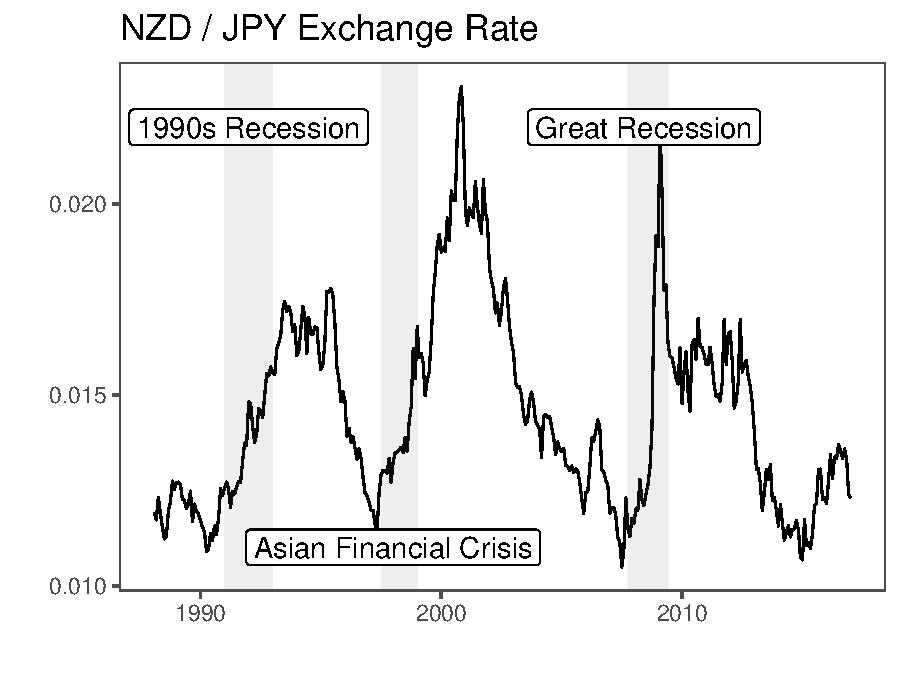
\includegraphics[width=0.7\textwidth]{Exhibits/Figure_FX_JPYNZD.pdf}
    \label{fig:spot}
\end{figure}
Continuing with our example from Figure \ref{fig:fp}, Figure \ref{fig:spot} plots the New
Zealand dollar - Japanese yen exchange rate in terms of dollars per
yen. An increase in the exchange rate indicates yen appreciation.
The shaded areas highlight three distinct periods of global economic
turmoil: The early 1990s recession (1990 - 1993), the Asian financial
crisis (1997 - 1998), and the Great Recession (2007 - 2009). In each of these periods, 
the yen appreciated markedly against the New Zealand Dollar. If these appreciations during periods of economic
turmoil are part of a broader pattern, investors should naturally consider the Japanese yen the safer
currency. Hence, the lower returns earned on Japanese yen investments 
may be a result of the yen's usefulness as a hedge against bad times. 
On the other hand, we should expect investing in the New Zealand dollar 
earns higher returns, because the New Zealand dollar provides none of 
the hedging benefits of the Japanese yen and is therefore a riskier 
currency for global investors.

\subsection{Reduced-form Evidence}

A large empirical asset pricing literature constructs \emph{risk-factors} to 
attribute cross-sectional differences in asset returns to different sources 
of risk by looking for comovement in asset returns \citep{Fama1976}. Typically, 
researchers sort assets based on some characteristic of interest, and then 
divides asset into a small number of portfolios based on the sort. The first 
portfolio typically contains assets with the lowest values of the characteristic of 
interest, and the last portfolio typically contains assets with the highest 
values. A risk factor is then constructed by taking the difference in returns 
between the fist and last portfolio. Researchers determine a risk factor 
explains asset returns by running regressions of returns on the risk factor, and 
showing that assets with higher regression coefficients on the risk factor also 
obtain higher expected returns.\footnote{For example, \citet{FamaFrench1992} 
constructed two risk factors by sorting U.S. equities into portfolios based on 
market capitalization and book-to-market ratio, and showed portfolios of stocks
with greater exposure to these two risk factors obtained higher average returns.}

% A key innovation of the empirical asset pricing literature is also to analyze 
% portfolio returns rather returns than on individual assets. Again, assets are 
% sorted into portfolios based on some dimension of interest. Intuitively, 
% averaging the returns of assets within portfolios eliminates diversifiable and 
% asset-specific risks. The remaining variation in returns across portfolios 
% should better capture the risk-return trade-off specifically from differing along
% the dimension of interest. 

In a seminal paper, \citet{LustigRoussanovVerdelhan2011} applied these asset
pricing techniques to exchange rates and provided systematic evidence that 
the greater returns obtained from investing in high-interest-rate currencies 
result from greater risk exposure. For every month between November 1983 and 
December 2009, the authors sorted currencies into 6 portfolios based 
on their risk-free rate differential relative to the U.S. dollar. The first 
portfolio contained currencies with the lowest risk-free rates and the 
last portfolio contained currencies with the highest risk-free rates. The 
authors constructed a \emph{carry trade} risk factor by taking the difference 
in the returns between the portfolio containing the highest-interest-rate 
currencies and the portfolio containing the lowest-interest-rate currencies.

\citet{LustigRoussanovVerdelhan2011} showed that differential exposure to 
their carry trade risk factor accounted the expected returns from investing 
in different currencies. The authors regressed the returns of their 6 
currency portfolios on their carry trade risk factor.
The portfolios with higher-interest-rate currencies obtained a higher average
return and also covaried more positively with the risk factor. An increase in 
the regression coefficient on the carry trade risk factor from 0 to 1 was 
associated with a large and highly significant increase of 5.5 percent per 
year. 

In this sense, \citet{LustigRoussanovVerdelhan2011} identified a common source
of risk in currency markets, and showed that exposure to this common source 
of risk explained cross-sectional differences in currency returns. However, 
the major drawback of this asset pricing method is that it does not reveal 
the ultimate source of risk. In other words, we know exchange rates move with 
each other, but we do not know the economic forces that drive this comovement.

Hence, many researchers have tried to identify relationships between currency 
returns and macro-financial variables to understand the source of currency risk. \citet{LustigVerdelhan2007} showed that low-interest-rate currencies provide a 
hedge against U.S. consumption growth risk. Low-interest-rate currencies 
systematically appreciate when U.S. consumption growth is low, and high-interest-rate 
currencies tend to depreciate when U.S. consumption growth is low. Thus, the 
U.S. investor can hedge against periods of low consumption growth by investing 
in a portfolio of low-interest-rate currencies. U.S. investors 
find this hedging property useful, and therefore accept a lower rate of return. 

Moreover, low-interest-rate currencies tend to appreciate during periods of 
financial turmoil, whereas high-interest-rate currencies tend to depreciate. \citet{LustigRoussanovVerdelhan2011}  and \citet{CampbellMedeirosViceira2010} 
showed low-interest-rate currencies tend to appreciate whenever equity markets 
are volatile. Consistent with this evidence, \citet{Menkhoffetal2012} measure 
of periods financial market turmoil using exchange rate data, and show 
low-interest-rate currencies provide a hedge against periods of high exchange 
rate volatility. 

Literature on crash risk:
\begin{itemize}
    \item \citet{Brunnermeieretal2009} studied eight major currencies. Higher 
    interest rate currencies exhibited greater chance of 
    large devaluations (i.e. crash risk).
    \item Jurek2014 - Constructs carry trades without crash risk to quantify the contribution of crash risk to carry trades. At most 1/3.
    \item Farhietal2015 -  Similar to Jurek. How much of the carry trade is driven by crash risk? Also arrives at around 1/3.
    \item Lewis2011 - peso problems (no risk premia, simply mismeasuring average returns due to small samples)
\end{itemize}

Each of these papers highlight different ways in which high-interest-rate currencies 
may be riskier than low-interest-rate currencies. However, the common thread among 
these papers is that the persistent differences in returns to investing in various
currencies reflect persistent differences in the stochastic properties of their 
exchange rates. Under this interpretation, currencies yielding lower returns are safer 
currencies that tend to appreciate during periods of economic distress. 


\subsection{Theory: Microfoundations of Safe Haven Currencies}

Prompted by this empirical evidence, the theoretical literature has identified several fundamental economic forces that may make a given currency safer or riskier from the perspective of global investors. Although there is an ongoing debate on which of these forces may be most important in practice, many of of these microfounded models share a common structure, which we can summarize using just a few key equations.

Consider a world economy in which international assets
are priced by the marginal utility of an international investor, $\lambda_T$, which will be our measure of ``good'' and ``bad'' times. Times are good when $\lambda_T$ is low, and times are bad when it is high. In different models, $\lambda_T$ may be the marginal utility of consumption of traded goods (the part of consumption that his shared internationally), the marginal utility of consumption of a key investor who intermediates between segmented international markets, or the capital constraint of such an intermediary. 
Households consume a country-specific final good, the price of which (accounted for in
a common unit) depends on $\lambda_T$ and a country-specific shock,
$x^n$,
\begin{equation}
  p^{n}=a\lambda _{T}+b x^{n}.  \label{eq_RF}
\end{equation}%
The country-specific shock
interchangeably may stem from a country-specific supply, demand, or monetary shock; in
other words, it is a stand-in for any factor that affects the price of
consumption in one country more than in others. The higher $x^{n}$,
the higher the price of domestic consumption relative to that in other countries. 
For simplicity, assume $\lambda _{T}\sim N(0,\sigma^2_{\lambda_{T}})$ and
$x^{n} \sim N(0,\sigma^2_x) $ are normally distributed, not
necessarily independent, shocks and $a$ and $b$ are constants greater
than zero.

The real exchange rate between two countries is the relative price of
their respective final goods. In logs,
\begin{equation}\label{eq_RER}
  s^{f,h}=p^{f}-p^{h}=b(x^{f}-x^{h}),
\end{equation}
where the second equality substitutes (\ref{eq_RF}).
Because of $x^{n}$, the relative price of consumption may differ between the two countries, allowing the real exchange rate to move. When the price of consumption in country $f$ increases, its consumption bundle appreciates relative to country $h$. In this sense, we can speak of ``currencies'' even without formally introducing money into the model. 

By definition, the risk-free bond in country $h$ pays $p^h$ with certainty, while that in country $f$ pays $p^f$ with certainty, so that each country's risk-free bond pays exactly one unit of that country's consumption bundle. Importantly, because the real exchange rate may move around, country $h$'s risk-free bond is not risk-free from the perspective of households in country $f$, and vice versa. For this reason, one country's risk-free bond may be more expensive than the other country's risk-free bond. The risk-free rate of interest is the yield to maturity of the risk-free bond, so that the country with the more expensive risk-free bond automatically must have the lower risk-free rate of interest. In this sense, any model with a variable real exchange rate as in equation (\ref{eq_RER}) may produce differences in risk-free interest rates across countries.

Different theories of such differences in interest rates apply
elementary asset pricing to equation (\ref{eq_RER}). One can show that the log expected return to
borrowing in country $h$ and to lending in country $f$ is
\begin{equation}
  r^{f} + \Delta \mathbb{E} s^{f,h} - r^{h} =cov\left( \lambda _{T},p^{h}-p^{f}\right),
  \label{eq_UIP_RF}
\end{equation}%
where $r^{n}$ is the risk-free interest rate in country $n$.\footnote{$\Delta\mathbb{E}s^{f,h}$ is defined as the
  logarithm of the ratio of the countries' expected real price
  changes. See Appendix \ref{Appendix_ReducedFormResults} for a formal
  derivation.} This statement means a currency that tends to
appreciate when $\lambda_T$ is high pays a lower expected return and,
if $\Delta \mathbb{E} s^{f,h}\approx0$ (as is the case in the data), therefore must has a lower risk-free interest
rate. That is, a currency that appreciates in bad times (for example, in times when
consumption goods are expensive everywhere) provides a
hedge against worldwide consumption risk and pays lower returns in
equilibrium.

Equations (\ref{eq_RF}) and (\ref{eq_UIP_RF}) are the main ingredients
of risk-based models of unconditional differences in interest rates
across countries, where different approaches have identified different reasons why the countries differ in the degree to which their price indices covary with $\lambda_T$.

\paragraph*{Country Size}




FIXMETH Describe
\begin{enumerate}
\item Hassan (2013)[MATH*]

\begin{equation} \lambda_{T}^\ast = -c
  \sum_{n} \theta^n x^n,
  \label{eqn:lambdat2NP}
\end{equation}
larger countries have lower interst rates
stock returns traded nontraded sector
Currency Union

\begin{equation}
  r^{f \ast} + \Delta \mathbb{E} s^{f, h \ast} - r^{h \ast}
  =g\left(\theta^h - \theta^f\right) \sigma_N^2.
  \label{eq_FF_UIP}
\end{equation}
\item Martin
\item Richmond (2019)

$$\lambda_{T}^\ast = -c
  \sum_{n} \theta^n x^n- d\sum_{n} \nu^n x^n$$



\item Ready Roussanov Ward (2017) (and Maggiori JMP?)
$$p^{\text{Commodity Country}}=a\lambda_T+b\frac{\text{Finished goods shipped}}{\text{Shipping Capacity}} $$
Commodity producers appreciate in good times and depreciate in bad times
Their exchange rates are positively correlated with the commodity price and shipping costs.
\item Farhi and Gabaix (2016)
Countries differ in their resilience to disaster risk. Conditional on a disaster striking the world economy, the currencies of more resilient countries appreciate. 
\item Gourinchas, Govillot and Rey: Differences in country size and risk aversion
\item Della Corte, Riddiough and Sarno (2016)
\item Tran (2013)
\item Powers (2015)
\item Wiriadinata (2020)
\end{enumerate}

\subsection{Evidence}

[Puzzle 1: microfoundation which is it]

If there is indeed something to this story, it changes how we think
about central issues in macro.



\section{The Interest Differential Puzzle}

[Puzzle 2]
[MATH?]

\section{Currency Risk and the allocation of capital across countries}
There are large differences in capital accumulation across countries:

Hassan, Mertens and Zhang (2016)
\begin{equation}\label{eq_link_k_r}
  k^{f\ast}-k^{h\ast} = \frac{\gamma}{\tau(\gamma-1)^2}\left(r^{h \ast} - \Delta \mathbb{E} s^{f, h \ast} - r^{f \ast}\right).
\end{equation}
Implication 1
\begin{enumerate}
\item Lucas (1988)
\end{enumerate}
Implication 2
\begin{enumerate}
\item Caselli and Feyrer (2007)
\item Monge-Naranjo, Sanchez and Santaeualia-Llopis (2018)
\end{enumerate}
Implication 3: corporate balance sheets
\begin{enumerate}
\item Richers (2020)
\item di Giovanni, Kalemli-Ozcan, Ulu, Baskaya (2019)
\item David, Henriksen and Simanovska
\end{enumerate} [picture]
\section{Currency Risk and Exchange Rate Regimes}
Q: Are there other papers that argue policies can manipulate risk
premia?
\begin{equation*}
  p^m = p^{m \ast} + (1 - \theta^m) \zeta (p^{t \ast} - p^{m \ast}).
\end{equation*}
\section{Current Accounts and the Reserve Currency Paradox}
 [Puzzle 3: Reserve Currency Paradox]
 [MATH*]

\section{Dynamics}

HABITS -Theory
Verdelhan (2010)
Heyerdahl-Larsen (2014)
Stathopoulos (2012)
LRR -Theory
Colacito and Croce (2011,2013)
Colacito, Croce, Ho and Howard (2018)
Bansal Shaliastovich (2013)
DISASTERS - Theory
Gourio, Siemer, Verdelhan (2013)
Guo (2010)
Du (2013)
Martin (2013)
Farhi and Gabaix
DISASTERS - Empirics


\subsection{Quantitative literature}
\begin{enumerate}
\item Colacito and Croce (2011)
\item Gourio, Siemer and Verdelhan (2013)
\item Colacito, Croce, Ho and Howard (2018)
\end{enumerate}
\subsection{Theories written for FPP}
Heyerdahl-Larsen Statopoulous Verdelhan Backus Foresi Telmer 
Bansal-Shaliastovich
Gabaix and Maggiori
\subsection{Measurement of risk}
Maybe measurement of risk - implied vol - commercial indices -
newspapers - conference call transcripts
\subsection{Global financial cycle}

\section{Capital flows and the allocation puzzle}
Capital flows run counter to neo-classical model:
\begin{enumerate}
\item Gourinchas and Jeanne (2013)
\item[-] Current explanations:
\item Differences in financial development (Ju and Wei, 2006;
  Caballero, Farhi and Gouinchas, 2008; Mendoza, Quadrini and
  Rios-Rull, 2009)
\item Differences in factor utilization (Jin, 2012)
\item Differences in contracting frictions (Aguiar and Amador, 2010)
\end{enumerate}

\section{Dynamics of Currency Risk Premia}


\section{Unsorted}
\begin{enumerate}
\item Gourinchas and Rey (2007)
\item Govillot, Rey and Gourinchas (2010)
\item[-] Implications for equilibrium portfolios and global imbalances
\item Miranda-Agrippino and Rey (2020)
\item[-] Global financial cycles
\item Boccola and Lorenzoni (forthcoming)
\item[-] Debt crises
\item Du and Schreger
\item[-] Corporate balance sheets
\item[-] Special role for the dollar
\item Hassan, Mertens and Zhang (2020)
\item Burnside, Eichenbaum, Kleshchelski and Rebelo (2011)
\end{enumerate}



\subsection{Sidebars and Margin Notes}
% Margin Note
\begin{marginnote}[]
\entry{Term A}{definition}
\entry{Term B}{definition}
\entry{Term C}{defintion}
\end{marginnote}

\begin{textbox}[h]\section{SIDEBARS}
Sidebar text goes here.
\subsection{Sidebar Second-Level Heading}
More text goes here.\subsubsection{Sidebar third-level heading}
Text goes here.\end{textbox}



\subsection{Equations}
% Example of a single-line equation
\begin{equation}
a = b \ {\rm ((Single\ Equation\ Numbered))}
\end{equation}
%Example of multiple-line equation
Equations can also be multiple lines as shown in Equations 2 and 3.
\begin{eqnarray}
c = 0 \ {\rm ((Multiple\  Lines, \ Numbered))}\\
ac = 0 \ {\rm ((Multiple \ Lines, \ Numbered))}
\end{eqnarray}

% Summary Points
\begin{summary}[SUMMARY POINTS]
\begin{enumerate}
\item Summary point 1. These should be full sentences.
\item Summary point 2. These should be full sentences.
\item Summary point 3. These should be full sentences.
\item Summary point 4. These should be full sentences.
\end{enumerate}
\end{summary}

% Future Issues
\begin{issues}[FUTURE ISSUES]
\begin{enumerate}
\item Future issue 1. These should be full sentences.
\item Future issue 2. These should be full sentences.
\item Future issue 3. These should be full sentences.
\item Future issue 4. These should be full sentences.
\end{enumerate}
\end{issues}

\newpage

\setstretch{1}

\bibliographystyle{chicago} \bibliography{ARE}

\clearpage


\appendix

\begin{center}
  {\Huge\bf Appendix}\\
  {\large\bf -For online publication only-}
\end{center}

\section{Derivation of Equation \ref{eq_UIP_RF} \label{Appendix_ReducedFormResults}}

The country $n$ risk-free bond pays off $P_n$ units of the traded good at maturity. We derive the value of the risk-free bond, $V_n$, by applying the asset pricing equation to the bond payoff: 
\begin{equation*}
  V_n = \mathbb{E}\left[M_{T} P_n
  \right],
\end{equation*}
where $M_{T}$ denotes the stochastic discount factor. The country $n$ risk-free rate (in levels), $R^f_n$, is the inverse of the price of the risk-free bond:
\begin{equation*}
  R^f_n = \frac{1}{V_n}.
\end{equation*}
Putting the previous two equations together yields the following relationship:
\begin{equation*}
  \mathbb{E}\left[ M_T P_n \right] R^f_n = 1.
\end{equation*}
As a result, the risk-free rates of countries $f$ and $h$ are related as follows:
\begin{equation*}
  \mathbb{E}\left[M_T P_f \right] R^f_f 
  = \mathbb{E}\left[M_T P_h \right] R^f_h = 1
\end{equation*} 
If the stochastic discount factor and prices are log-normal, we can perform the following calculations:
\begin{align*}
  & \mathbb{E}\left[M_{T} P_f \right] R^f_f
    = \mathbb{E}\left[M_{T} P_h \right] R^f_h \\
  \Leftrightarrow\quad
  & \mathbb{E}\left[\exp\left[ m_T + p_f + r^f_f \right]\right]
    = \mathbb{E}\left[\exp\left[ m_T + p_h + r^f_h \right]\right] \\
  \Leftrightarrow\quad
  & \mathbb{E}\left[m_T + p_f\right] + \frac{1}{2}\text{var}\left(m_T\right) +      \frac{1}{2}\text{var}\left(p_f\right) + \text{cov}\left(m_{T}, p_f\right) + r^f_f \\
  & = \mathbb{E}\left[m_{T}+ p_h\right] + \frac{1}{2}\text{var}\left(m_{T}\right) + \frac{1}{2}\text{var}\left(p_h\right) + \text{cov}\left(m_T, p_h\right) + r^f_h,
\end{align*}
We cancel out $\text{var}\left( m_T \right)$ from both sides of the previous equation.
\begin{align*}
  & \mathbb{E}\left[p_f\right]+\frac{1}{2}\text{var}\left(p_f\right) + \text{cov}\left(m_T, p_f\right) + r^f_f = \mathbb{E}\left[p_h\right]+\frac{1}{2}\text{var}\left(p_h\right)+\text{cov}\left(m_T,p_h\right) + r^f_h
  \\      \Leftrightarrow \quad
  & r^f_f+\mathbb{E}\left[p_f-p_h\right]+\frac{1}{2}\text{var}\left(p_f\right)-\frac{1}{2}\text{var}\left(p_h\right)-r^f_h = -\text{cov}\left(m_T,p_f-p_h\right)\\   
  \Leftrightarrow\quad
  &r^f_f+\log\left(\mathbb{E}\left[P_f\right]/\mathbb{E}\left[P_h\right]\right)-r^f_h = -\text{cov}\left(m_T,p_f-p_h\right)
\end{align*}
We define
$\Delta\mathbb{E}\left[s_{f,h}\right]
=\log\left(\mathbb{E}\left[P_f\right]/\mathbb{E}\left[P_h\right]\right).$
With this definition:
\begin{equation*} 
  r^f_f+\Delta\mathbb{E}\left[s_{f,h}\right]-r^f_h = -\text{cov}\left(m_T,p_f-p_h\right). 
\end{equation*}

\section{Derivation of Equation \ref{eq_BFT} \label{Appendix_BFT}}

Letting $M_n$ denote the stochastic discount factor measured in units of the consumption bundle specific to country $n$ and assuming no arbitrage, we know the risk-free rate in country $n$ satisfies:
\begin{equation*}
    R^f_n = \frac{1}{\mathbb{E} \left[ M_n\right] }
\end{equation*}
If we further assume $M_n$ is log-normally distributed, then
\begin{eqnarray*}
r^f_n &=&-\log \left( E\left[ M_n \right] \right)  \\
&=&-\left( E\left[ m_n \right] +\frac{1}{2}\text{var}\left[ m_n \right] \right) 
\end{eqnarray*}
Next, take the difference between the risk-free rates of countries $f$ and $h$:
\begin{eqnarray*}
r^f_f - r^f_h  
&=& -\left( \mathbb{E} \left[ m_f \right] +\frac{1}{2}\text{var}\left[ m_f \right] \right) 
+ \left( \mathbb{E}\left[ m_h \right] +\frac{1}{2}\text{var}\left[ m_h \right] \right)  \\
r^f_f-r^f_h + \mathbb{E} \left[ m_f - m_h \right] 
&=& \frac{1}{2}\left( \text{var}\left[ m_h \right] - \text{var}\left[ m_f \right] \right) 
\end{eqnarray*}
Finally, when financial markets are complete, $\Delta s_{f, h} = m_f - m_h$. Thus
\begin{eqnarray*}
r^f_f + \mathbb{E} \Delta s_{f, h} - r^f_h 
&=& \frac{1}{2}\left( \text{var}\left[ m_h \right] - \text{var}\left[ m_f \right] \right)
\end{eqnarray*}
    

\end{document}